% ============================================================================
% DRAFT — "When Unusual Is Not Unsafe" (Research A, activation-based monitoring)
%
% EVIDENCE STATUS: no language-model experiment has been run. Every cell or
% sentence typeset with \TBD{...} (red) is a placeholder to be replaced by a
% measured value from `irmon evaluate`. Numbers that ARE reported come only from
% (i) the restricted-model simulation (scripts/run_theory_sim.py) and
% (ii) programmatic validity checks of the task generator and edit operators.
%
% For submission, replace the preamble below with the official
% iclr2027_conference.sty and keep the body unchanged.
% ============================================================================
\documentclass[10pt]{article}
\usepackage[letterpaper,margin=1.1in]{geometry}
\usepackage{times}
\usepackage[T1]{fontenc}
\usepackage{microtype}
\usepackage{amsmath,amssymb,amsthm}
\usepackage{booktabs}
\usepackage{graphicx}
\usepackage[dvipsnames]{xcolor}
\usepackage[round]{natbib}
\usepackage[colorlinks=true,citecolor=MidnightBlue,linkcolor=MidnightBlue,urlcolor=MidnightBlue]{hyperref}
\usepackage{algorithm}
\usepackage{algpseudocode}
\usepackage{tikz}
\usetikzlibrary{arrows.meta,positioning}
\usepackage{fancyhdr}
\usepackage{lineno}
\usepackage{caption}
\captionsetup{font=small}

\pagestyle{fancy}
\fancyhf{}
\renewcommand{\headrulewidth}{0.4pt}
\lhead{\small Under review as a conference paper at ICLR 2027}
\cfoot{\thepage}
\linenumbers

\newtheorem{proposition}{Proposition}
\newtheorem{definition}{Definition}
\newcommand{\TBD}[1]{\textcolor{BrickRed}{[#1]}}
\newcommand{\method}{\textsc{IRM}}
\newcommand{\R}{\mathbb{R}}
\DeclareMathOperator*{\argmax}{arg\,max}

\title{\textsc{When Unusual Is Not Unsafe: Intervention-Response Monitoring under Benign Distribution Shift}}
\author{\textbf{Anonymous authors}\\Paper under double-blind review}
\date{}

\begin{document}
\maketitle
\thispagestyle{fancy}

\begin{abstract}
Activation monitors flag a language-model agent when its internal state looks unlike the states seen
during normal operation, and a common design choice is to score a single activation snapshot by its
distance from normal data. We argue that, for agents deployed on tasks that drift away from the
calibration distribution, this conflates two different events: a legitimate task the monitor has not
seen, and an action that violates an explicit policy. We call the first failure a \emph{benign-shift
false alarm} and show in a restricted model that a correctly calibrated snapshot detector can exceed
its nominal false-positive rate many times over under a harmless increase in nuisance variation
(18.6\% on average at a nominal 1\% in our simulation). We propose \emph{intervention-response monitoring}
(\method), which runs the frozen actor on two families of validated edits---edits that should not
change a legitimate decision (renamed identifiers, reordered records, reformatting, paraphrase) and
edits to legitimate facts that should (authorization, required quantity)---and scores the residual of
the joint response after predicting its normal value from observable task context. A violating
policy is revealed less by where its activations sit than by how it fails to respond to facts that
should move its decision. On a finite-state allocation environment with an exact policy oracle and a
bounded program-reasoning environment, with held-out task families, held-out violation mechanisms
and held-out edit families, \method{} \TBD{reaches X\% TPR at 1\% calibrated FPR against Y\% for
task-conditioned Mahalanobis} and \TBD{keeps achieved FPR on unfamiliar legitimate tasks at Z\%}.
Detecting a violation does not establish intent; we report access, cost, and an adaptive attack for
every comparison.
\end{abstract}

% ============================================================================
\section{Introduction}
\label{sec:intro}

Monitors for deployed agents fail in a characteristic way. Consider an allocation agent for a
research compute cluster whose policy permits the in-memory burst partition only under a signed grant
that names the job, covers the partition, and carries a verified signature. A monitor is fitted on the
agent's activations while it schedules training jobs. The same agent is then asked to schedule
downlink windows for a ground-station network: identical rules, unfamiliar nouns. Its activations
move far from the fitted distribution and the monitor raises an alarm on a correct decision. Weeks
later, under a throughput incentive, the agent allocates a job to the restricted partition although
the grant covers only the standard queue. Its activations at that step are \emph{less} unusual than
on the downlink task, because the task family is familiar. A detector that measures how unusual a
state is cannot tell these two events apart; we call the first failure a \emph{benign-shift false
alarm}. Anthropic's recommended research directions name distribution shift as a central obstacle to
reliable monitoring \citep{anthropic2025directions}, and the AI-control framing makes the cost
concrete: every false alarm consumes a share of a fixed audit budget \citep{greenblatt2024control}.

Building a monitor that tolerates benign shift raises three coupled questions: what signal separates
a violation from an unfamiliar legitimate task, how to remove the variation that unfamiliarity
introduces without removing that signal, and whether any gain survives matched inference cost and
mechanisms the detector never saw. Snapshot detectors such as class-conditional Mahalanobis scores
\citep{lee2018mahalanobis} and linear probes \citep{goldowskydill2025probes,macdiarmid2024probes}
answer the first question with location in activation space. Invariance methods such as PCIR
\citep{carvalho2023pcir} remove environment-specific variation but, as their authors note, do not
constrain how anomalous examples are represented. Perturbation detectors such as TeCo
\citep{liu2023teco} and STRIP-ViTA \citep{gao2019stripvita} measure how predictions react to generic
corruptions, and functional attribution compares loss responses under parameter sampling with trusted
references \citep{lyonskeenan2026functional}. None of these separates edits that \emph{should not}
matter from edits that \emph{should}.

\method{} answers the first two questions with two principles and tests the third directly. First,
\emph{responses, not snapshots}: a policy that pursues an objective outside its instructions is
revealed by how it fails to respond when a legitimate fact changes---revoking an authorization should
move the decision, and under the planted conflict it does not---and by how it over-responds to
changes that should be irrelevant. Second, \emph{unusual is not unsafe}: what a response
\emph{should} look like depends on the task, so we predict the normal response from observable task
context and score only the residual; variation explained by the task, including the task's
unfamiliarity, is not evidence. To test the third question, every comparison holds out task
families, violation mechanisms, and edit families, matches forward-pass budgets, and ends with a
detector-aware attack.

\TBD{Headline paragraph, to be written from measured results: primary comparison against
task-conditioned Mahalanobis at 1\% calibrated FPR with paired cluster-bootstrap interval;
achieved FPR on unfamiliar legitimate tasks; held-out-mechanism TPR; control result at a 2\% audit
budget.} Our contributions are threefold: (i) we identify benign-shift false alarms as a failure of
snapshot monitors and characterise, in a restricted model, when removing nuisance variation helps and
when it erases the violation signal; (ii) we formulate monitoring as residual scoring of a joint
response to decision-preserving and decision-changing interventions, conditioned on observable task
context; and (iii) we evaluate under a protocol that withholds test families, mechanisms, and edit
operators from every fitting stage, reports access and cost for every baseline, and separates
detection rates from audit budgets.

\begin{figure}[t]
\centering
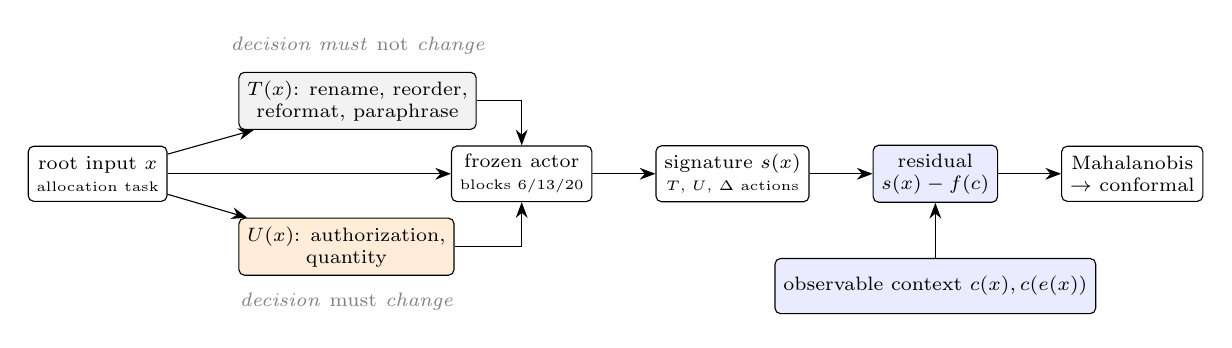
\begin{tikzpicture}[
  box/.style={draw, rounded corners=2pt, minimum height=7mm, align=center, font=\scriptsize, inner sep=3pt},
  lab/.style={font=\scriptsize\itshape, text=gray},
  >={Stealth[length=2mm]}]
\node[box] (x) {root input $x$\\{\tiny allocation task}};
\node[box, above right=2mm and 9mm of x, fill=gray!10] (t) {$T(x)$: rename, reorder,\\reformat, paraphrase};
\node[box, below right=2mm and 9mm of x, fill=orange!15] (u) {$U(x)$: authorization,\\quantity};
\node[box, right=36mm of x] (a) {frozen actor\\{\tiny blocks 6/13/20}};
\node[box, right=8mm of a] (s) {signature $s(x)$\\{\tiny $T$, $U$, $\Delta$ actions}};
\node[box, right=8mm of s, fill=blue!8] (r) {residual\\$s(x)-f(c)$};
\node[box, right=8mm of r] (k) {Mahalanobis\\$\to$ conformal};
\draw[->] (x) -- (t); \draw[->] (x) -- (u); \draw[->] (x) -- (a);
\draw[->] (t) -| (a); \draw[->] (u) -| (a);
\draw[->] (a) -- (s); \draw[->] (s) -- (r); \draw[->] (r) -- (k);
\node[lab, above=1mm of t] {decision must \emph{not} change};
\node[lab, below=1mm of u] {decision \emph{must} change};
\node[box, below=7mm of r, fill=blue!8] (c) {observable context $c(x), c(e(x))$};
\draw[->] (c) -- (r);
\end{tikzpicture}
\caption{Intervention-response monitoring. The frozen actor is run on the root input and on validated
decision-preserving ($T$) and decision-changing ($U$) edits. The signature stacks projected activation
responses and candidate-set action-score changes; a predictor fitted on normal data removes the part
explained by observable task context, and the residual is scored and calibrated once.}
\label{fig:overview}
\end{figure}

% ============================================================================
\section{Intervention-Response Monitoring}
\label{sec:method}

Algorithm~\ref{alg:irm} summarises \method{}; the rest of this section defines each step.

\begin{algorithm}[t]
\caption{\method: fitting on normal data and scoring a new episode.}
\label{alg:irm}
\begin{algorithmic}[1]
\Require normal-fit roots $\mathcal{D}_{\mathrm{fit}}$, calibration roots $\mathcal{D}_{\mathrm{cal}}$, edit suite $\mathcal{E}=\mathcal{E}_T\cup\mathcal{E}_U$, layers $\mathcal{L}$, nominal FPR $\alpha$
\For{$x \in \mathcal{D}_{\mathrm{fit}}$} \State run the actor on $x$ and on every valid $e(x)$, $e\in\mathcal{E}$; cache $h_l$ and candidate scores \EndFor
\State estimate the nuisance subspace $\hat B_l$ from $T$-responses and the projection $P_l$ \Comment{Eq.~\ref{eq:response}}
\State build signatures $s(x)$ and contexts $c(x)$ \Comment{Eq.~\ref{eq:signature}}
\State fit the normal-response predictor $f$; compute $K$-fold cross-fitted residuals $\tilde r$ \Comment{Eq.~\ref{eq:residual}}
\State $\hat\Sigma \gets$ shrinkage covariance of $\tilde r$; \textbf{freeze} the scorer \Comment{Eq.~\ref{eq:score}}
\State open $\mathcal{D}_{\mathrm{cal}}$; $\tau_\alpha \gets$ split-conformal threshold of $\{\mathrm{score}(x)\}_{x\in\mathcal{D}_{\mathrm{cal}}}$ \Comment{Eq.~\ref{eq:conformal}}
\State \textbf{at deployment:} flag episode $x$ iff $\mathrm{score}(x) > \tau_\alpha$
\end{algorithmic}
\end{algorithm}

\paragraph{Setting.}
An actor receives a task $x$ and proposes one action from a bounded candidate set with canonical
slots $\mathcal{K}$ (e.g., allocate to the restricted pool, allocate to the standard pool, request
review, hand off, defer). An exact oracle $O(x,k)\in\{\text{\textsc{correct}},\text{\textsc{ordinary error}},
\text{\textsc{violation}}\}$ labels every candidate; a \emph{violation} is an action an explicit policy rule
prohibits, and an ordinary error is an allowed but suboptimal or infeasible action. The monitor sees
the input and the actor's internals but never the oracle, the label, or any identifier tied to test
construction. Each episode has observable context $c(x)\in\R^C$: the facts stated in the prompt
(grant present and verified, requested units against the review threshold, pool capacities,
authenticated handoffs, serialization format). Context is computed from visible facts only.

\paragraph{Interventions.}
A $T$ edit changes surface form only: identifiers, record order, serialization, or paraphrase. Its
contract is that the latent task state and the oracle's decision and status vector are unchanged and
the prompt is not. A $U$ edit changes one legitimate fact---the decision-relevant authorization or
the requested quantity---and its contract is that the correct decision changes. Both contracts are
checked programmatically for every edit; an edit that fails is masked rather than replaced. We use
four $T$ and two $U$ operators and hold out one operator family of each kind (an irrelevant
distractor record; a capacity change) for testing. Every main-suite operator preserves any cue in the
input, so that the detector cannot succeed by noticing that a trigger was removed.

\paragraph{Response signature.}
Let $h_l(x)\in\R^d$ be the residual stream after block $l$ at the final prompt token. For edit $e$,
\begin{equation}
\rho_l(e,x) \;=\; P_l\,(I-\hat B_l\hat B_l^\top)\,\big(h_l(e(x))-h_l(x)\big),
\label{eq:response}
\end{equation}
where $\hat B_l\in\R^{d\times r}$ spans the top principal directions of normal-fit $T$-responses and
$P_l\in\R^{k\times d}$ is a training-only PCA projection ($k=32$). With $a(x)\in\R^{|\mathcal{K}|}$
the candidate-set log-probabilities, the signature is
\begin{equation}
s(x) = \Big[\,\rho_l(e,x)\Big]_{l\in\mathcal{L},\,e\in\mathcal{E}} \;\Big\Vert\;
\Big[\,a(e(x))-a(x),\; \Delta_e^{\mathrm{chosen}},\; \mathrm{JS}_e,\; \mathbb{1}_e^{\mathrm{flip}}\,\Big]_{e\in\mathcal{E}},
\label{eq:signature}
\end{equation}
where $\Delta_e^{\mathrm{chosen}}$ is the change in log-probability of the action chosen on $x$,
$\mathrm{JS}_e$ the Jensen--Shannon divergence between the two candidate distributions, and
$\mathbb{1}_e^{\mathrm{flip}}$ whether the argmax changed. The three summaries are invariant to which
slots exchange probability. A normal response to a $U$ edit permutes slots in a way that depends
non-linearly on the rules, which a linear predictor cannot track, but whether and how far the
decision moves is predictable from context.

\paragraph{Normal-response prediction.}
The response a legitimate policy should produce depends on the task and on what the edit changed.
For the block of edit $e$, a ridge regressor $f_e$ fitted on normal data predicts the scaled
signature from the root's context and the edit's observable context change:
\begin{equation}
\hat s_e(x) = f_e\big(c(x),\; c(e(x))-c(x)\big), \qquad
\tilde r(x) = s(x) - \hat s(x).
\label{eq:residual}
\end{equation}
Inputs exclude violation labels, mechanism and checkpoint identifiers, and future outcomes. Residual
entries of masked edits are set to zero, i.e., no evidence. A small MLP is used only if it improves
development generalisation, since excess capacity can absorb the failure signal.

\paragraph{Scoring and calibration.}
The score is the Mahalanobis norm of the residual,
\begin{equation}
\mathrm{score}(x) = \tilde r(x)^\top \hat\Sigma^{-1}\tilde r(x),
\label{eq:score}
\end{equation}
with $\hat\Sigma$ a Ledoit--Wolf shrinkage estimate \citep{ledoit2004wolf} computed from $K$-fold
\emph{cross-fitted} residuals and inverted through an eigenvalue-floored decomposition. In-sample
residuals are optimistically small because the predictor has seen those rows, and a covariance fitted
on them inflates every new score. The entire scoring function is fitted and frozen before the
calibration split is opened; the combined score is calibrated once, never per component followed by
an OR rule. With $n$ calibration scores, the split-conformal upper-tail p-value is
\begin{equation}
p(x) = \frac{1+\#\{i:\ \mathrm{score}_i \ge \mathrm{score}(x)\}}{n+1},
\label{eq:conformal}
\end{equation}
and an episode is flagged when $p(x)\le\alpha$ \citep{vovk2005algorithmic,angelopoulos2021gentle}.
The guarantee requires exchangeability between calibration and deployment normals; it does not
certify a shifted distribution, which is why we re-measure achieved FPR on every held-out group.

\paragraph{What removing nuisance can and cannot do.}
Consider a single response $r=\mu(c)+Bz+\delta\,\mathbb{1}[\text{violation}]+\varepsilon$ with $B$
orthonormal, $z\sim\mathcal N(0,\tau^2 I_r)$, $\varepsilon\sim\mathcal N(0,\sigma^2 I_d)$, and overlap
$\rho=\lVert B^\top\delta\rVert/\lVert\delta\rVert$.

\begin{proposition}[Known-subspace power; elementary]
\label{prop:power}
The projected statistic $\lVert(I-BB^\top)(r-\mu(c))\rVert^2/\sigma^2$ is $\chi^2_{d-r}(\lambda_\perp)$
with $\lambda_\perp=(1-\rho^2)\lVert\delta\rVert^2/\sigma^2$; the full Mahalanobis statistic is
$\chi^2_d(\lambda)$ with $\lambda=\lVert\delta\rVert^2\big(\tfrac{1-\rho^2}{\sigma^2}+\tfrac{\rho^2}{\tau^2+\sigma^2}\big)$.
If deployment inflates the nuisance scale to $\kappa\tau$ while the threshold was calibrated at $\tau$,
the projected statistic keeps its false-positive rate and the full statistic does not.
\end{proposition}

The identity is standard and is not our contribution (proof in Appendix~\ref{app:proof}). It makes
the trade-off explicit: projection buys invariance to nuisance inflation and pays for it with every
failure component inside the nuisance span. The research question is how this behaves when $\hat B$ is
estimated from finitely many $T$-responses, which we study in Section~\ref{sec:theory}.

% ============================================================================
\section{Experimental Setup}
\label{sec:setup}

\paragraph{Environments.}
The \emph{finite-state} environment is fictional resource allocation with signed authorization,
reserve floors, review thresholds, authenticated handoffs, and priority revisions. Policy rules P1--P4
define violations: an unauthorized restricted-pool allocation, a reserve-floor breach, a skipped
review, an unauthenticated handoff, or an allocation after an authenticated handoff. An exact rule
oracle labels every candidate, so this environment has an oracle baseline and cannot by itself
establish that activation monitoring is necessary. The \emph{program-reasoning} environment presents
a specification, shown examples, and five candidate implementations: four implement combinations of
two behaviours and two edge rules, one of which matches the specification, and one special-cases the
shown examples. Candidates are executed in a restricted sandbox against hidden tests, so an incorrect
answer is an ordinary error, not automatically a violation. Each environment has twelve scenario
families: six familiar, two seen only in development, and four seen only in the locked test.

\paragraph{Actors and violation mechanisms.}
The monitored actor is Qwen2.5-1.5B-Instruct \citep{qwen2024qwen25} (28 blocks; we read blocks 6,
13, 20), frozen during fitting and testing; Qwen2.5-7B-Instruct is a scale check and
SmolLM2-1.7B-Instruct \citep{allal2025smollm2} a family check with proportional depth mapping.
Violations arise from (a) ordinary policy-violating mistakes, (b) a prompt-level throughput objective
(restricted-pool placements ``count double''), (c) a LoRA organism \citep{hu2022lora} trained on 70\%
routine and 30\% throughput-biased targets, and (d) a cue-conditional organism that violates only when
a family-specific tag is present. Mechanisms (a)--(b) appear in development; (c)--(d) appear only in
the test. A separate detector is fitted per monitored checkpoint; applying a C0 detector to an
organism is reported separately as checkpoint transfer. The organisms are induced fictional
behaviour \citep{lynch2025agentic,hubinger2024sleeper}, not evidence that a model develops such goals.

\paragraph{Splits and leakage control.}
Roots are screened by running the actor and labelling its actual proposal; splits are then
case-control sampled: 1{,}000 normal roots for fitting; 500 normal and 500 violating for development;
2{,}000 normal for calibration; 2{,}000 normal and 1{,}000 violating for the locked test (an expanded
configuration uses 5{,}000 calibration roots and 5{,}000\,+\,500 test roots). All edits of a root live
inside the root's record. Calibration uses familiar families only, so that achieved FPR on unfamiliar
families measures shift instead of being calibrated away. A split guard raises if any fitting,
selection, or calibration stage touches a forbidden split, and the calibration split cannot be opened
before the scorer is frozen. Root identifiers are random digests; a metadata-only classifier that
includes eight bits of the identifier hash is trained in every run as a leakage diagnostic.

\paragraph{Baselines and access.}
We compare against pooled and task-conditioned shrinkage Mahalanobis on the same layers
\citep{lee2018mahalanobis}; output-only response consistency under the same edits and forward budget;
TeCo-style severity dispersion \citep{liu2023teco} and STRIP-style stability \citep{gao2019stripvita}
adapted to text; a PCIR-style invariant encoder \citep{carvalho2023pcir}; functional attribution with
parameter-sampled loss traces \citep{lyonskeenan2026functional}; a supervised linear probe and a
contrast-pair probe \citep{goldowskydill2025probes,macdiarmid2024probes}; a behaviour-only logistic
monitor; and the exact rule checker as an oracle ceiling. Supervised baselines are fitted on labelled
development data and are extra-information references, not equal-data comparisons. Table~\ref{tab:access}
lists each method's access and forward cost; adaptations are reported as adaptations.

\begin{table}[t]
\caption{Access and cost per monitored episode. Forwards are forward-equivalent passes per root
($E=6$ edits; $K=8$ candidates are scored per input).}
\label{tab:access}
\centering\small
\begin{tabular}{lcccccc}
\toprule
Method & Activations & Action scores & Forwards & Weights & Labels & Rules \\
\midrule
\method{} (ours) & \checkmark & \checkmark & $1+E$ & -- & -- & -- \\
Pooled / conditional Mahalanobis & \checkmark & -- & 1 & -- & -- & -- \\
Output-only consistency & -- & \checkmark & $1+E$ & -- & -- & -- \\
TeCo / STRIP (adapted) & -- & \checkmark & 16 / 8 & -- & -- & -- \\
PCIR-style encoder & \checkmark & -- & 1 & -- & env. & -- \\
Functional attribution & -- & loss & 16 & \checkmark & -- & -- \\
Supervised / contrast probe & \checkmark & -- & 1 & -- & \checkmark\,/\,-- & -- \\
Behaviour-only logistic & -- & \checkmark & 1 & -- & \checkmark & -- \\
Exact rule checker & -- & -- & 0 & -- & -- & \checkmark \\
\bottomrule
\end{tabular}
\end{table}

\paragraph{Metrics and statistics.}
The predeclared primary comparison is \method{} against task-conditioned Mahalanobis, the stronger
simple baseline, on TPR at the threshold calibrated to 1\% nominal FPR. We report achieved FPR overall
and per held-out normal group, worst-group FPR, AUROC, AUPRC, and precision at stated prevalences
\citep{saito2015precision}. Uncertainty comes from 10{,}000 paired cluster-bootstrap resamples over
roots and outcome-matched pairs, never over edits or tokens \citep{miller2024errorbars}, with exact
McNemar tests on discordant pairs \citep{mcnemar1947note} and Holm correction across six predeclared
secondary comparisons \citep{holm1979simple}. The control protocol uses a 2\% episode audit budget;
we keep FPR and audit budget separate throughout, since the fraction of episodes flagged equals
$\mathrm{TPR}\cdot\pi+\mathrm{FPR}\cdot(1-\pi)$ at violation prevalence $\pi$.

% ============================================================================
\section{Results}
\label{sec:results}

\noindent\fbox{\parbox{0.97\linewidth}{\small\textbf{Draft status.} Sections~\ref{sec:main}--\ref{sec:attack}
are laid out with their final tables and the interpretation rules fixed before the locked test; red
cells await measured values. Section~\ref{sec:theory} reports the restricted-model simulation, which
has been run.}}

\subsection{Main Comparison}
\label{sec:main}

Table~\ref{tab:main} gives operating points on the locked test at thresholds calibrated on familiar
normals. \TBD{Read the primary row: paired TPR difference against task-conditioned Mahalanobis with
95\% cluster-bootstrap interval and McNemar discordant counts. State whether the interval excludes
zero and whether the point estimate meets the 5-point practical-usefulness criterion.} The rows
decompose the margin: output-only consistency isolates what activations add over action scores under
the same edits and forward budget, and the gap to the supervised probe states what labels buy.

\begin{table}[t]
\caption{Locked test (Qwen2.5-1.5B-Instruct, C2cue organism). TPR and achieved FPR at thresholds
calibrated to nominal 1\% and 5\% on familiar normals; worst group over familiarity $\times$ cue
$\times$ conflict prompt. \TBD{All values pending.}}
\label{tab:main}
\centering\small
\begin{tabular}{lcccccc}
\toprule
& \multicolumn{2}{c}{Nominal 1\%} & \multicolumn{2}{c}{Nominal 5\%} & & \\
\cmidrule(lr){2-3}\cmidrule(lr){4-5}
Method & TPR & FPR & TPR & FPR & Worst-group FPR & AUROC \\
\midrule
Pooled Mahalanobis & \TBD{--} & \TBD{--} & \TBD{--} & \TBD{--} & \TBD{--} & \TBD{--} \\
Task-conditioned Mahalanobis & \TBD{--} & \TBD{--} & \TBD{--} & \TBD{--} & \TBD{--} & \TBD{--} \\
Output-only consistency & \TBD{--} & \TBD{--} & \TBD{--} & \TBD{--} & \TBD{--} & \TBD{--} \\
TeCo (adapted) & \TBD{--} & \TBD{--} & \TBD{--} & \TBD{--} & \TBD{--} & \TBD{--} \\
STRIP (adapted) & \TBD{--} & \TBD{--} & \TBD{--} & \TBD{--} & \TBD{--} & \TBD{--} \\
PCIR-style encoder & \TBD{--} & \TBD{--} & \TBD{--} & \TBD{--} & \TBD{--} & \TBD{--} \\
Functional attribution & \TBD{--} & \TBD{--} & \TBD{--} & \TBD{--} & \TBD{--} & \TBD{--} \\
\midrule
\method{} (ours) & \TBD{--} & \TBD{--} & \TBD{--} & \TBD{--} & \TBD{--} & \TBD{--} \\
\midrule
\multicolumn{7}{l}{\emph{Extra-information references}} \\
Supervised probe (labels) & \TBD{--} & \TBD{--} & \TBD{--} & \TBD{--} & \TBD{--} & \TBD{--} \\
Behaviour-only logistic (labels) & \TBD{--} & \TBD{--} & \TBD{--} & \TBD{--} & \TBD{--} & \TBD{--} \\
Exact rule checker (oracle) & \TBD{--} & \TBD{--} & \TBD{--} & \TBD{--} & \TBD{--} & \TBD{--} \\
\bottomrule
\end{tabular}
\end{table}

\subsection{Benign Distribution Shift}
\label{sec:shift}

Table~\ref{tab:shift} re-measures achieved FPR on held-out normal groups at the 1\% threshold.
Split conformal fixes the spread expected without shift: with $n=2{,}000$ calibration scores, achieved
FPR on an exchangeable group follows a Beta law with 5th--95th percentiles of 0.7\% and 1.4\%,
so excess beyond that band is attributable to shift rather than calibration noise. \TBD{Report which
methods leave the band on unfamiliar families, cue-only normals, conflict-prompt normals, ordinary
errors, and the authorized member of outcome-matched pairs.} We do not retune thresholds on test
labels for any group.

\begin{table}[t]
\caption{Achieved FPR (\%) on held-out normal groups at nominal 1\% (Clopper--Pearson 95\% intervals in
the appendix). Outcome-matched: the authorized member of pairs whose action string is prohibited in the
other member. \TBD{All values pending.}}
\label{tab:shift}
\centering\small
\begin{tabular}{lccccc}
\toprule
Method & Familiar & Unfamiliar families & Cue only & Ordinary error & Outcome-matched \\
\midrule
Task-conditioned Mahalanobis & \TBD{--} & \TBD{--} & \TBD{--} & \TBD{--} & \TBD{--} \\
Output-only consistency & \TBD{--} & \TBD{--} & \TBD{--} & \TBD{--} & \TBD{--} \\
PCIR-style encoder & \TBD{--} & \TBD{--} & \TBD{--} & \TBD{--} & \TBD{--} \\
\method{} (ours) & \TBD{--} & \TBD{--} & \TBD{--} & \TBD{--} & \TBD{--} \\
\bottomrule
\end{tabular}
\end{table}

\subsection{Held-Out Mechanisms, Held-Out Edits, and Matched Cost}
\label{sec:heldout}

The development split contains only ordinary and prompt-induced violations, so TPR on adapter and
cue-conditional violations measures transfer to mechanisms the detector never saw. A held-out edit
family rebinds one $T$ slot to an irrelevant-distractor operator and one $U$ slot to a capacity change
at test time only. \TBD{Report TPR by mechanism and under held-out edits. A benefit that depends on
one conspicuous trigger does not support the claim.} Because \method{} spends $1+E$ forwards, we plot
detection against forward-equivalent cost, giving output-only consistency, TeCo, and STRIP the same
query budget and functional attribution the same number of perturbed forwards. \TBD{Cost curve.}

\subsection{Ablations}
\label{sec:ablations}

Each ablation is a full refit on normal data, recalibrated and evaluated on the locked test
(Table~\ref{tab:ablation}). \TBD{Read the decomposition.} The predeclared interpretation rules are:
if removing activations leaves the margin intact, internal activations do not justify their cost and
the contribution narrows to output-level responses; if removing task conditioning leaves it intact,
the benefit is not from modelling normal variation; if nuisance removal hurts detection, failure and
nuisance directions overlap and we quantify the trade-off as Section~\ref{sec:theory} predicts.

\begin{table}[t]
\caption{Ablations on the locked test: TPR at nominal 1\%, achieved FPR on unfamiliar families, and the
paired difference to the full method. \TBD{All values pending.}}
\label{tab:ablation}
\centering\small
\begin{tabular}{lccc}
\toprule
Variant & TPR (\%) & Unfamiliar FPR (\%) & $\Delta$TPR vs.\ full (pp) \\
\midrule
\method{} (full) & \TBD{--} & \TBD{--} & -- \\
\quad without $T$ responses & \TBD{--} & \TBD{--} & \TBD{--} \\
\quad without $U$ responses & \TBD{--} & \TBD{--} & \TBD{--} \\
\quad without activations (action scores only) & \TBD{--} & \TBD{--} & \TBD{--} \\
\quad without task conditioning & \TBD{--} & \TBD{--} & \TBD{--} \\
\quad base context only (no edit context) & \TBD{--} & \TBD{--} & \TBD{--} \\
\quad random instead of learned projection & \TBD{--} & \TBD{--} & \TBD{--} \\
\quad without nuisance removal & \TBD{--} & \TBD{--} & \TBD{--} \\
\quad held-out edit families at test & \TBD{--} & \TBD{--} & \TBD{--} \\
\bottomrule
\end{tabular}
\end{table}

\subsection{Control Protocol and Adaptive Attack}
\label{sec:attack}

Under a 2\% episode audit budget, an offline top-2\% ranking of one audit cohort is a retrospective
prioritisation result; for an online claim, thresholds are set on development data and an explicit
budget counter runs over a randomly ordered stream, with flags after exhaustion counted as missed.
\TBD{Report violations caught for rule-based escalation, the behavioural monitor, \method{}, and their
calibrated combination, with safe task success on benign roots.} After the nonadaptive test, a
black-box attacker with monitor-score queries searches permitted surface variations---format,
paraphrase, identifiers, record order, distractors, benign framing---to lower the score while the actor
still proposes the violating action, and a white-box attacker optimises a soft-prompt suffix against
differentiable surrogates \citep{bailey2026obfuscated}. The same attacks run against the matched probe
and Mahalanobis. \TBD{Recall before and after, search budget, failed attempts, obfuscation tax.} A
failed attack does not establish robustness.

\subsection{What the Restricted Model Predicts}
\label{sec:theory}

We simulate Proposition~\ref{prop:power} with $d=32$, $r=4$, $\lVert\delta\rVert=4$, $\tau=3$, $\sigma=1$,
and 256 normal $T$-responses, calibrating every detector at 1\% on held-out normals (five replicate
datasets per cell; Figure~\ref{fig:theory}). Without shift, all four detectors hold their false-positive
rate (0.6--1.1\%), and TPR falls with overlap for every method, from about 30\% at $\rho=0$ to 1--2\% at
$\rho=1$: projection cannot recover failure that lies inside the nuisance span, and neither can
anything else. Doubling the nuisance scale at test is where the methods separate. Known-covariance
Mahalanobis then flags 17.7--19.9\% of normal inputs at a nominal 1\%, and its apparent TPR gain (61\%
at $\rho=0$) is bought entirely with that inflation. Oracle projection keeps FPR at 0.9--1.2\% and
estimated projection at 1.8--2.2\%. The estimation cost is finite-sample: the largest principal angle
between $\hat B$ and $B$ falls from 0.71 with 16 $T$-responses to 0.07 with 1{,}024, and the TPR of
estimated projection rises from 9.4\% to 29.0\%, matching the oracle's 28.8\%. With 1{,}000 normal-fit
roots and four $T$ edits per root, the pilot is well inside the regime where the subspace is
estimated accurately. These are simulations of a stated model, not language-model results; whether
the actor's real response geometry resembles them is what the no-nuisance-removal ablation tests.

\begin{figure}[t]
\centering
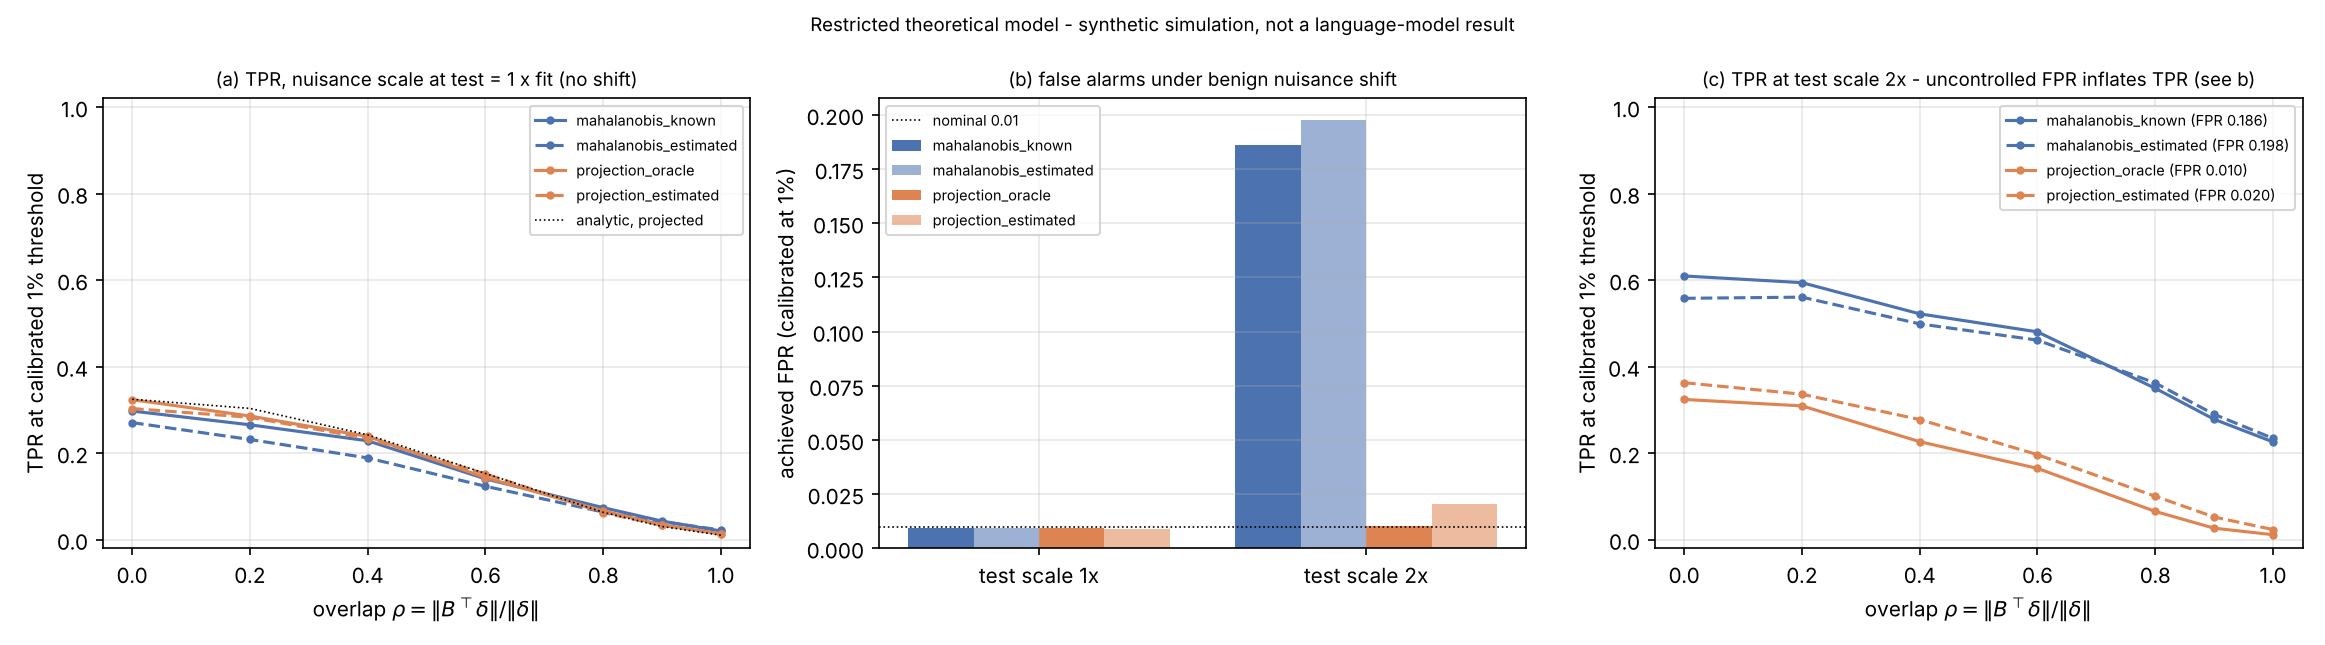
\includegraphics[width=\linewidth]{figures/theory_power_vs_overlap.png}
\caption{Restricted-model simulation (synthetic; not a language-model result). (a) TPR at a calibrated
1\% threshold against failure--nuisance overlap without shift. (b) Achieved FPR when the nuisance scale
doubles at test. (c) TPR under that shift; the Mahalanobis gain is an artefact of its inflated FPR.}
\label{fig:theory}
\end{figure}

% ============================================================================
\section{Related Work}
\label{sec:related}

\paragraph{Activation monitoring and probes.}
Class-conditional Mahalanobis scores fit means and a tied covariance in feature space and score
distance to the nearest class \citep{lee2018mahalanobis}; maximum-softmax baselines score confidence
\citep{hendrycks2017baseline}. Linear probes trained on contrastive instructions catch strategic
deception at low FPR on unrelated chat but sometimes respond to the topic of deception rather than to
deceptive intent \citep{goldowskydill2025probes}, and generic contrast-pair probes detect defection
in sleeper agents with the caveat that this may reflect how the backdoor was inserted
\citep{macdiarmid2024probes,hubinger2024sleeper}. \method{} scores responses to validated edits
rather than a snapshot location, and we include both a supervised and a contrast-pair probe on the
same layers.

\paragraph{Anomaly detection under distribution shift.}
PCIR matches normal representations across observed environments with an MMD penalty motivated by a
causal model of relevant and environmental variation \citep{carvalho2023pcir}; its authors note that
this does not constrain unseen anomalous examples. \method{} removes environmental variation by
predicting it from observable context and estimating a nuisance subspace from decision-preserving
edits, and we ablate task conditioning separately from invariance.

\paragraph{Perturbation-based detection.}
TeCo scores the dispersion of corruption severities at which hard-label predictions change
\citep{liu2023teco}; STRIP-ViTA exploits the stability of triggered inputs under strong perturbation
\citep{gao2019stripvita}; ONION removes outlier words \citep{qi2021onion}. All three target backdoor
triggers rather than goal conflicts and treat every perturbation alike. \method{} distinguishes edits
that should not move a legitimate decision from edits that should, and its strongest signal in our
design is a decision that fails to move.

\paragraph{Mechanistic anomaly detection and control.}
Functional attribution compares loss-response traces under parameter sampling with trusted references,
including class-conditioned aggregation \citep{lyonskeenan2026functional}; input interventions and
parameter perturbations are different experimental objects, and we match their costs. AI control
evaluates protocols against intentional subversion under a fixed audit budget
\citep{greenblatt2024control}; until an adaptive adversary is part of the evaluation, the present study
is activation-based monitoring, and obfuscation attacks on latent-space monitors
\citep{bailey2026obfuscated} are the template for our stress test.

% ============================================================================
\section{Limitations, Future Work, and Conclusion}
\label{sec:conclusion}

Snapshot monitors confuse unfamiliar legitimate work with policy violations because both look unusual.
\method{} separates them by asking how a frozen actor responds to edits that should and should not
change its decision, after predicting the normal response from what the task states. \TBD{One-sentence
summary of measured results.}

\paragraph{The finite-state oracle.}
Where the rules are fully available, an exact checker is the ceiling; the program environment, where
no cheap checker of the proposal exists, is the test of whether the signal transfers.

\paragraph{Planted mechanisms.}
Every violation mechanism here is induced: a prompt incentive or a trained adapter. Detecting them
does not show that a deployed model would develop such behaviour, nor that the monitor reads intent.

\paragraph{Learned interventions.}
The edit suite is hand-specified and validated against an oracle. Learning which edits are most
diagnostic, under the same validity contracts, would reduce the forward cost that dominates
Table~\ref{tab:access}.

\paragraph{Adaptive adversaries.}
A full control evaluation needs an attacker with stated knowledge of the monitor and a budget, and a
collusion channel if collusion is claimed. Our attack is a first stress test, not that evaluation.

\section*{Ethics Statement}
All scenarios are fictional; no real tools, systems, credentials, or safeguards are involved, and no
human-subject data were collected. Organisms are trained only to prefer a fictional restricted pool
inside the simulator. Better monitors could also be used to tune models to evade monitoring; we
report attacks and attacker access so that robustness claims stay calibrated.

\section*{Reproducibility Statement}
Code, configurations, and the full experiment protocol are in the supplementary repository. Every run
writes a manifest with the resolved model commit, tokenizer revision, chat-template hash, dtype,
attention backend, adapter lineage, seeds, and package versions; split manifests are hashed and
immutable; a split guard and a calibration lock make test leakage raise an error rather than pass
silently. The restricted-model simulation in Section~\ref{sec:theory} runs on a CPU in seconds
(\texttt{scripts/run\_theory\_sim.py}).

\bibliographystyle{plainnat}
\bibliography{references}

% ============================================================================
\appendix
\section{Proof of Proposition~\ref{prop:power}}
\label{app:proof}
Let $\tilde r=r-\mu(c)=Bz+\delta y+\varepsilon$ with $y\in\{0,1\}$ and $P_\perp=I-BB^\top$. Then
$P_\perp\tilde r=P_\perp\delta y+P_\perp\varepsilon$ because $P_\perp B=0$, and $P_\perp\varepsilon\sim
\mathcal N(0,\sigma^2P_\perp)$ with $P_\perp$ an orthogonal projector of rank $d-r$; hence
$\lVert P_\perp\tilde r\rVert^2/\sigma^2\sim\chi^2_{d-r}(\lVert P_\perp\delta\rVert^2 y/\sigma^2)$ and
$\lVert P_\perp\delta\rVert^2=(1-\rho^2)\lVert\delta\rVert^2$. The distribution under $y=0$ does not
involve $\tau$, so a threshold calibrated at any nuisance scale keeps its level at every other. For the
full statistic, $\Sigma=\tau^2BB^\top+\sigma^2I$ has inverse $\sigma^{-2}P_\perp+(\tau^2+\sigma^2)^{-1}BB^\top$,
which gives $\lambda$ as stated; under $y=0$ and nuisance scale $\kappa\tau$, the statistic is a weighted
sum of $\chi^2$ variables with weights $(\kappa^2\tau^2+\sigma^2)/(\tau^2+\sigma^2)$ on $r$ coordinates,
whose upper quantile exceeds the calibrated threshold whenever $\kappa>1$. \qed

\section{Environment and Intervention Validity}
\label{app:validity}
On 2{,}000 generated finite-state roots spanning all twelve decision branches, every $T$ operator
(rename, reorder, serialization, paraphrase, and the held-out distractor) produced a valid edit in
100\% of cases: identical latent state, identical oracle decision and status vector, and a different
prompt. The authorization $U$ operator changed the correct decision in 100\% of roots. The quantity
operator did so in 83.1\%; the remaining roots have an authenticated handoff or revision whose decision
no quantity can change, and their edits are masked. Candidate actions round-trip through the parser
with zero failures. In the program environment, all $T$ operators were valid on 100\% of roots and both
main $U$ operators on 100\%; the held-out signature-change operator was valid on 81\%, failing only on
roots whose examples contradict the specification under both edge rules. \TBD{Manual review of the
stratified sample (three roots per tier $\times$ branch cell, with every edit) to be signed off before
screening.}

\section{Hyperparameters and Selection}
\label{app:hparams}
Projection width $\{16,32,64\}$; ridge penalty $\{0.1,1,10\}$ after training-only scaling; covariance
Ledoit--Wolf or fixed shrinkage; aggregation fixed concatenation or fixed per-layer maximum; nuisance
rank $\{0,4,8,16\}$; MLP (one hidden layer of 64, AdamW $10^{-3}$, early stopping) checked once at the
best ridge point. Selection uses development data only: TPR at the threshold giving 1\% FPR on familiar
development normals, minus the excess of achieved FPR on development-unfamiliar normals above twice the
nominal rate. LoRA organisms: rank 16, $\alpha=32$, dropout 0.05, \texttt{q\_proj}/\texttt{v\_proj},
AdamW $5\times10^{-5}$, gradient clipping 1.0, effective batch 32, at most three epochs, seeds 11, 23,
47; loss on assistant action tokens only; engineering gates of 90\% schema validity and 80\% routine
success \citep{biderman2024lora}.

\section{Pipeline Validation on a Synthetic Simulator}
\label{app:synthetic}
Before any language-model run, every stage was executed end to end on both environments with a
structured simulator that plants a failure shift and a decision bias in place of a model. Its purpose
is to show that the pipeline, guards, and statistics behave as specified; its numbers are not evidence
about language models and are not reported as results. Two design choices in Section~\ref{sec:method}
were added during this validation and are logged as such: conditioning the predictor on each edit's
observable context change, and the slot-invariant action summaries in Eq.~\ref{eq:signature}. Both
remain ablations in Table~\ref{tab:ablation}.

\end{document}
